\subsection{Where full cost penalization lost accuracy}
Table~\ref{tab:length} shows why fewer calls alone were insufficient. At 33 or more tokens, the teacher got 186/208 correct versus 174/208 for the student. Calling the teacher on all 208 would fix 18 errors and introduce six. Confidence-only recovered nine of the twelve net corrections with 45 calls. The original cost-aware gate sent just 13 of these cases and recovered five net corrections. For requests with positive estimated gain, dividing by a larger cost suppresses their score even when the teacher often helps in that group.

\begin{table}[H]
\centering
\caption{Full-model correctness and routed teacher calls by token length on the 872 GLUE SST-2 sentences. The student is the four-layer distilled FP32 model. Original and tuned use cost exponents 1 and 0.16 respectively.}
\label{tab:length}
\setlength{\tabcolsep}{5pt}
\begin{tabular}{rrrrrrr}
\toprule
 & & \multicolumn{2}{c}{Correct if used alone} & \multicolumn{3}{c}{Teacher calls}\\
\cmidrule(lr){3-4}\cmidrule(l){5-7}
Tokens & Cases & Student & Teacher & Original & Confidence & Tuned\\
\midrule
3--16 & 197 & 185 & 183 & 33 & 17 & 11\\
17--32 & 467 & 406 & 425 & 75 & 99 & 88\\
33+ & 208 & 174 & 186 & 13 & 45 & 50\\
\bottomrule
\end{tabular}
\end{table}

Softening the cost exponent to 0.75 raised the original frozen policy from 779 to 786 correct and increased calls on the longest group from 13 to 35. Its total calls rose from 121 to 161. At a common offline budget of 161, the original, softened, and confidence rankings got 782, 786, and 789 correct, respectively. The fixed softened rule met the one-point accuracy budget, and five paired CPU runs showed mixed timing results. The wider continuous exponent sweep found no stable interval that improved on confidence-only at equal calls on both short-text splits.

\subsection{Grid search, latency, and transfer}
Of 4,641 fixed-cutoff policies, 186 met the GLUE accuracy, call, and estimated cost conditions. Only seven beat confidence-only accuracy, all by one example (Figure~\ref{fig:grid}). The GLUE choice used exponent 0.10 and cutoff 0.09240. It used 20 fewer calls on GLUE, then lost three correct predictions on Stanford while making 45 fewer calls. The two-split choice used exponent 0.16 and cutoff 0.07545. It preserved the Stanford count with 28 fewer calls (Table~\ref{tab:transfer}). Stanford's labels helped select the 0.16 policy, so the tie is retrospective.

\begin{figure}[H]
  \centering
  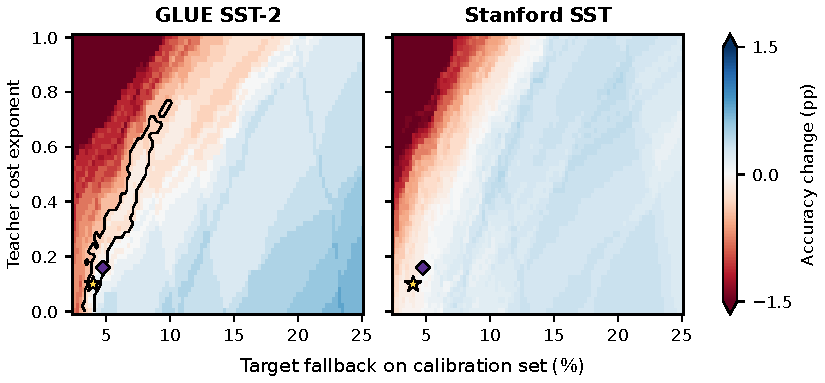
\includegraphics[width=\linewidth]{report/figures/gate-grid.pdf}
  \caption{Accuracy change in percentage points (pp) relative to confidence-only on two short-text splits. Blue indicates gains and red indicates losses. Black contours outline the eligible GLUE grid cells. The star marks the GLUE-only choice and the diamond marks the two-split choice. A target sets a fixed calibration score cutoff, so realized call rates vary by split.}
  \label{fig:grid}
\end{figure}

\begin{table}[H]
\centering
\caption{Correct predictions and teacher calls for the same fixed cutoffs on GLUE, Stanford, and previously unscored IMDb reviews. Each cell gives correct predictions followed by calls.}
\label{tab:transfer}
\begin{tabular}{lrrr}
\toprule
Policy & GLUE (872) & Stanford (1,812) & IMDb (720)\\
\midrule
Confidence-only & 789 / 161 & 1,670 / 337 & 647 / 147\\
GLUE choice, \(\alpha=0.10\) & 790 / 141 & 1,667 / 292 & 643 / 213\\
Two-split choice, \(\alpha=0.16\) & 790 / 149 & 1,670 / 309 & 643 / 213\\
\bottomrule
\end{tabular}
\end{table}

In the separate four-block timing run, the 0.16 gate made 12 fewer calls on the same workload and got one more prediction right. The median of process medians was 10.46 ms for the tuned gate and 10.53 ms for confidence-only. The corresponding p95 summaries were 29.46 and 28.67 ms. Within-block median latency fell in three pairs and rose in one, for a median paired change of \(-2.02\%\). The p95 rose in three pairs, for a median paired change of \(+3.14\%\) (Figure~\ref{fig:paired}). These relative changes summarize the paired blocks and therefore differ from ratios of the two aggregate latencies. Peak working sets were 928.0 and 927.7 MiB, respectively. Every timed prediction and route matched the replay. The tuned gate routed five more 33+ token requests and 17 fewer shorter requests than confidence-only. Timing aggregates do not identify whether this shift caused the higher p95.

\begin{figure}[H]
  \centering
  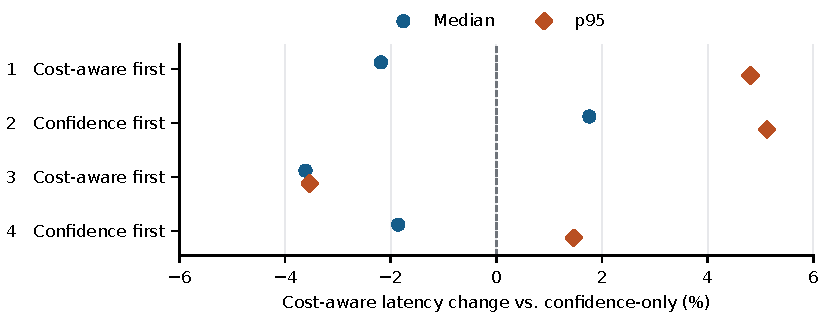
\includegraphics[width=\linewidth]{report/figures/paired-latency.pdf}
  \caption{Within-block latency changes for the frozen 0.16 policy relative to confidence-only. Each row compares the two policies on the same 872 requests in separate processes. Values left of zero favor the 0.16 gate. Markers show process-level estimates and first-policy order, with no request-level confidence intervals.}
  \label{fig:paired}
\end{figure}

On the 720-review IMDb audit, the two tuned policies made identical decisions. They included every confidence-only fallback plus 66 more. The extra calls fixed three student mistakes and introduced seven new ones. The net loss was four correct predictions (\(-0.56\) points, descriptive paired 95\% interval \([-1.39,+0.28]\) points). In this sample 718 reviews fell into the single 33+ token cost bin, where changing the exponent only rescales the predicted-gain scores. The fixed cutoff and gain model therefore determined the transfer outcome within almost the entire sample. IMDb and Stanford were accuracy and routing evaluations, without measured request latency for these policies.

\subsection{Alternative routing signals}
I screened additional formulas that shrank the length and interaction terms, applied additive cost, or used predicted class. The best GLUE formula only gained one correct prediction over confidence-only at 161 calls, then lost one at equal calls on the separate Stanford set. On a separate 720-review IMDb sample, two frozen scores using margin and length each gained one correct prediction at 174 calls by avoiding the same teacher-induced error. On another 960-review sample, a fix-minus-harm score matched confidence-only at 222 calls. Its fixed cutoff scored 867/960 with 206 calls versus 865/960 with 222 for the original confidence cutoff. At an offline confidence budget of 206 calls, the advantage narrowed to one correct prediction. These point results show where a policy can improve by avoiding teacher errors and also how much of an apparent gain depends on the operating point.
